%% METADATA
%% subject-code: DI01000061
%% subject-name: Modern Physics
%% semester: 1
%% examination: Winter-2024
%% date: 09-01-2025
%% description: Solution guide for Modern Physics (DI01000061)
%% tags: study-material, solutions, gtu, DI01000061, physics
%% END METADATA

\documentclass{article}

% content/resources/templates/preamble.tex
\usepackage[margin=0.6in]{geometry}
\author{Milav Dabgar}
\usepackage{amsmath,amssymb,amsthm}
\usepackage{booktabs}
\usepackage{multirow}
\usepackage{xcolor}
\usepackage{tcolorbox}
\tcbuselibrary{breakable,skins}
\usepackage[colorlinks=true,linkcolor=blue]{hyperref}
\usepackage{titlesec}
\usepackage{enumitem}
\usepackage{tikz}
\usepackage{pgfplots}
\usepackage{circuitikz}
\usepackage[version=4]{mhchem}
\usepackage{longtable}
\usepackage{array}
\usepackage{float}
\usepackage{caption}
\usepackage{listings}

\lstset{
  basicstyle=\small\ttfamily,
  breaklines=true,
  breakatwhitespace=false,
  postbreak=\mbox{\textcolor{red}{$\hookrightarrow$}\space},
  float=false,
  numbers=left,
  numberstyle=\tiny\color{gray},
  numbersep=10pt,
  xleftmargin=2em,
  keywordstyle=\color{blue},
  commentstyle=\color{green!60!black},
  stringstyle=\color{purple},
  backgroundcolor=\color{gray!5},
  showstringspaces=false,
  tabsize=2,
  captionpos=b,
  keepspaces=true,
  columns=flexible
}

\pgfplotsset{compat=1.18}
\usetikzlibrary{shapes,arrows,positioning,calc,patterns,decorations.pathmorphing,decorations.markings,arrows.meta}

% Color scheme
\definecolor{headcolor}{RGB}{0,102,204}
\definecolor{keycolor}{RGB}{220,20,60}
\definecolor{solutioncolor}{RGB}{34,139,34}
\definecolor{mnemoniccolor}{RGB}{148,0,211}
\definecolor{codecolor}{RGB}{0,0,100}

% Spacing
\setlength{\parskip}{3pt}
\setlist[itemize]{nosep}
\setlist[enumerate]{nosep}

% Title formatting
\titleformat{\section}{\Large\bfseries\color{headcolor}}{\thesection}{1em}{}
\titleformat{\subsection}{\large\bfseries\color{headcolor}}{\thesubsection}{1em}{}

% Pandoc tightlist compatibility
\providecommand{\tightlist}{%
  \setlength{\itemsep}{0pt}\setlength{\parskip}{0pt}}

% Pandoc longtable compatibility
\newcounter{none}
\def\thenone{}


\title{Modern Physics (DI01000061) - Winter 2024 Solution}
\date{January 9, 2025}

\hypersetup{
  pdftitle={Modern Physics (DI01000061) - Winter 2024 Solution},
  pdfsubject={GTU Exam Solution - Winter-2024},
  pdfauthor={Milav Dabgar},
  pdfkeywords={study-material, solutions, gtu, DI01000061, physics},
  pdfcreator={pdflatex}
}

\begin{document}
\maketitle

\setcounter{tocdepth}{5}
\tableofcontents
\newpage

% ========================================
% QUESTION 1: MCQs and Fill in the Blanks (14 marks)
% Demonstrates: Short answer format, multiple topics
% ========================================

\section{Question 1}
\textbf{Fill in the blanks/MCQs using appropriate choice from the given options.}

\subsection{Question 1(1) [1 marks]}
\textbf{Which of the following is a semiconductor?}

\textbf{Options:} (a) Si (b) Cu (c) Fe (d) Ni

\subsubsection{Solution}
\paragraph{Answer:} (a) Si

\paragraph{Explanation:}
Silicon (Si) is a Group 14 element with 4 valence electrons, making it an intrinsic semiconductor. Copper (Cu), Iron (Fe), and Nickel (Ni) are metals with high electrical conductivity due to free electrons.

\subparagraph{Note:} Germanium (Ge) is also a semiconductor from Group 14.

\paragraph{Mnemonic:} \emph{Si = Semiconductor, Cu/Fe/Ni = Metals.}

\subsection{Question 1(2) [1 marks]}
\textbf{Refractive index of glass is \_\_\_\_\_.}

\textbf{Options:} (a) 1.50 (b) 1.33 (c) 1.00 (d) 2.43

\subsubsection{Solution}
\paragraph{Answer:} (a) 1.50

\paragraph{Explanation:}
The refractive index of ordinary glass is approximately 1.50. Water has \(n = 1.33\), air/vacuum has \(n = 1.00\), and diamond has \(n = 2.43\).

\subparagraph{Note:} Higher refractive index means light travels slower in that medium.

\paragraph{Mnemonic:} \emph{Glass = 1.5, Water = 1.33, Diamond = 2.43.}

\subsection{Question 1(3) [1 marks]}
\textbf{When an angle of incidence becomes \_\_\_\_\_ critical angle, total internal reflection occurs.}

\textbf{Options:} (a) equal to (b) greater than (c) less than (d) none of these

\subsubsection{Solution}
\paragraph{Answer:} (b) greater than

\paragraph{Explanation:}
Total Internal Reflection (TIR) occurs when light travels from denser to rarer medium and the angle of incidence \(i\) is greater than the critical angle \(C\), i.e., \(i > C\).

\paragraph{Mnemonic:} \emph{TIR when i > C (Greater than Critical).}

\subsection{Question 1(4) [1 marks]}
\textbf{How many P-N junction diodes are used in a Bridge rectifier?}

\textbf{Options:} (a) 2 (b) 3 (c) 4 (d) 5

\subsubsection{Solution}
\paragraph{Answer:} (c) 4

\paragraph{Explanation:}
A bridge rectifier uses 4 diodes arranged in a bridge configuration to convert AC to full-wave DC. This allows current flow through the load in the same direction during both half cycles.

\paragraph{Mnemonic:} \emph{Bridge = 4 Diodes.}

\subsection{Question 1(5) [1 marks]}
\textbf{Optical fiber works on the principle of \_\_\_\_\_.}

\textbf{Options:} (a) Interference (b) Refraction (c) Polarization (d) Total internal reflection

\subsubsection{Solution}
\paragraph{Answer:} (d) Total internal reflection

\paragraph{Explanation:}
Optical fibers transmit light signals by repeated total internal reflection at the core-cladding interface, where the core has a higher refractive index than the cladding.

\paragraph{Mnemonic:} \emph{Fiber = TIR (Total Internal Reflection).}

\subsection{Question 1(6) [1 marks]}
\textbf{Number of oscillations performed per unit time is called \_\_\_\_\_.}

\textbf{Options:} (a) periodic time (b) wavelength (c) amplitude (d) frequency

\subsubsection{Solution}
\paragraph{Answer:} (d) frequency

\paragraph{Explanation:}
Frequency (\(f\)) is defined as the number of complete oscillations per unit time. Its unit is Hertz (Hz) or \(s^{-1}\). The relationship is \(f = 1/T\), where \(T\) is the periodic time.

\paragraph{Mnemonic:} \emph{Frequency = Oscillations per second.}

\subsection{Question 1(7) [1 marks]}
\textbf{The S.I. unit of electric charge is \_\_\_\_\_.}

\textbf{Options:} (a) Coulomb (b) Ampere (c) Volt (d) Faraday

\subsubsection{Solution}
\paragraph{Answer:} (a) Coulomb

\paragraph{Explanation:}
The SI unit of electric charge is Coulomb (C). One Coulomb is the charge transported by a current of one Ampere in one second (\(1\,C = 1\,A \times 1\,s\)).

\paragraph{Mnemonic:} \emph{Charge = Coulomb (C).}

\subsection{Question 1(8) [1 marks]}
\textbf{If the periodic time of simple pendulum is 2 second, then its frequency will be \_\_\_\_\_.}

\textbf{Options:} (a) 2 Hz (b) 0.5 Hz (c) 0.2 Hz (d) 5 Hz

\subsubsection{Solution}
\paragraph{Answer:} (b) 0.5 Hz

\paragraph{Explanation:}
The relationship between frequency (\(f\)) and periodic time (\(T\)) is inverse. Frequency tells us how many complete cycles occur per second, while period tells us how long one cycle takes.

\paragraph{Calculation:}
\[ f = \frac{1}{T} = \frac{1}{2} = 0.5 \, \text{Hz} \]

\paragraph{Mnemonic:} \emph{f = 1/T.}

\subsection{Question 1(9) [1 marks]}
\textbf{The velocity of light is \_\_\_\_\_ in vacuum.}

\textbf{Options:} (a) 300000 km/s (b) 300000 m/s (c) 341 km/s (d) 341 m/s

\subsubsection{Solution}
\paragraph{Answer:} (a) 300000 km/s

\paragraph{Explanation:}
The speed of light in vacuum is \(c = 3 \times 10^8\,m/s = 300000\,km/s\). This is a fundamental constant in physics. Note: 341 m/s is the speed of sound in air.

\paragraph{Mnemonic:} \emph{c = 3\texttimes10\textsuperscript{8} m/s = 300000 km/s.}

\subsection{Question 1(10) [1 marks]}
\textbf{The velocity of sound waves is maximum in \_\_\_\_\_.}

\textbf{Options:} (a) liquid (b) solid (c) gas (d) vacuum

\subsubsection{Solution}
\paragraph{Answer:} (b) solid

\paragraph{Explanation:}
Sound travels fastest in solids due to closely packed molecules and strong intermolecular forces. Order: \(v_{solid} > v_{liquid} > v_{gas}\). Sound cannot travel in vacuum.

\paragraph{Mnemonic:} \emph{Solids = Fastest sound.}

\subsection{Question 1(11) [1 marks]}
\textbf{The propagation of light wave is due to \_\_\_\_\_.}

\textbf{Options:} (a) crest and trough (b) compression and rarefaction (c) only compression (d) only rarefaction

\subsubsection{Solution}
\paragraph{Answer:} (a) crest and trough

\paragraph{Explanation:}
Light waves are transverse electromagnetic waves that propagate through alternating crests and troughs. Compression and rarefaction are associated with longitudinal waves like sound.

\paragraph{Mnemonic:} \emph{Light = Transverse = Crest/Trough.}

\subsection{Question 1(12) [1 marks]}
\textbf{LASER radiation is \_\_\_\_\_.}

\textbf{Options:} (a) polychromatic (b) monochromatic (c) low intense (d) none of these

\subsubsection{Solution}
\paragraph{Answer:} (b) monochromatic

\paragraph{Explanation:}
LASER (Light Amplification by Stimulated Emission of Radiation) produces monochromatic light, meaning it has a single precise wavelength. It is also coherent and highly intense.

\paragraph{Mnemonic:} \emph{LASER = Monochromatic, Coherent, Directional.}

\subsection{Question 1(13) [1 marks]}
\textbf{Which fiber provides longer bandwidth?}

\textbf{Options:} (a) Single mode (b) Multi mode step index (c) Step index (d) None of these

\subsubsection{Solution}
\paragraph{Answer:} (a) Single mode

\paragraph{Explanation:}
Single mode fibers have a very small core diameter and allow only one mode of light propagation, resulting in minimal dispersion and maximum bandwidth. They are used for long-distance communication.

\paragraph{Mnemonic:} \emph{Single mode = Long distance, High bandwidth.}

\subsection{Question 1(14) [1 marks]}
\textbf{What is value of acceptance angle of optical fiber having numerical aperture 0.5?}

\textbf{Options:} (a) \(30^\circ\) (b) \(45^\circ\) (c) \(60^\circ\) (d) \(15^\circ\)

\subsubsection{Solution}
\paragraph{Answer:} (a) \(30^\circ\)

\paragraph{Explanation:}
The acceptance angle is the maximum angle at which light can enter the optical fiber and still propagate through total internal reflection. It depends on the numerical aperture, which is a measure of the fiber's light-gathering ability.

\paragraph{Calculation:}
Numerical Aperture (NA) is related to acceptance angle (\(\theta_a\)) by:
\[ NA = \sin(\theta_a) \]
\[ 0.5 = \sin(\theta_a) \]
\[ \theta_a = \sin^{-1}(0.5) = 30^\circ \]

\paragraph{Mnemonic:} \emph{NA = sin(acceptance angle).}

% ========================================
% QUESTION 2: Theory Questions (14 marks)
% Q2(A): 3 marks each, Q2(B): 4 marks each
% ========================================

\section{Question 2}

\subsection{Question 2(a)(1) [3 marks]}
\textbf{Differentiate between accuracy and precision.}

\subsubsection{Solution}
\paragraph{Comparison Table:}
\begin{table}[H]
\caption{Accuracy vs Precision}
\centering
\begin{tabularx}{\textwidth}{|X|X|}
\hline
\textbf{Accuracy} & \textbf{Precision} \\ \hline
Closeness to true/standard value & Closeness of measurements to each other \\ \hline
Indicates correctness of measurement & Indicates reproducibility/consistency \\ \hline
Depends on systematic errors & Depends on least count of instrument \\ \hline
High accuracy = Low error & High precision = Values clustered together \\ \hline
Example: Hitting bullseye center & Example: Arrows grouped together \\ \hline
\end{tabularx}
\end{table}

\paragraph{Key Points:}
\begin{itemize}
    \item A measurement can be precise without being accurate (consistently wrong values)
    \item A measurement can be accurate without being precise (scattered around true value)
    \item Ideal measurement is both accurate AND precise
\end{itemize}

\paragraph{Example:}
If true value = 10.0 cm:
\begin{itemize}
    \item High accuracy, high precision: 10.0, 10.1, 9.9 cm (close to true, clustered)
    \item Low accuracy, high precision: 8.0, 8.1, 7.9 cm (wrong but consistent)
    \item High accuracy, low precision: 10.0, 12.0, 8.0 cm (average correct, scattered)
\end{itemize}

\paragraph{Mnemonic:} \emph{Accuracy = Correctness, Precision = Consistency.}

\subsection{Question 2(a)(2) [3 marks]}
\textbf{Determine the diameter of a sphere measured by micrometer screw, main scale reading is 5 mm and 50th division of circular scale is coinciding with base line. The least count of this instrument is 0.01 mm.}

\subsubsection{Solution}
\paragraph{Given Data:}
\begin{itemize}
    \item Main Scale Reading (MSR) = 5 mm
    \item Circular Scale Division (CSD) = 50
    \item Least Count (LC) = 0.01 mm
\end{itemize}

\paragraph{Formula:}
For a micrometer screw gauge, the total reading is the sum of the main scale reading and the product of the circular scale division and least count:
\[ \text{Reading} = \text{MSR} + (\text{CSD} \times \text{LC}) \]
The main scale reading gives the integral millimeters, while the circular scale gives the fractional part. The least count (0.01 mm) means each circular scale division represents 0.01 mm. When the 50th division coincides with the baseline, it indicates an additional 0.50 mm beyond the main scale reading.

\paragraph{Calculation:}
\[ \text{Diameter} = 5 + (50 \times 0.01) \]
\[ \text{Diameter} = 5 + 0.50 = 5.50 \, \text{mm} \]

\paragraph{Answer:}
The diameter of the sphere is \textbf{5.50 mm}. This measurement has a precision of ±0.01 mm due to the least count of the instrument.

\paragraph{Mnemonic:} \emph{MSR + (CSD × LC) = Total Reading.}

\subsection{Question 2(a)(3) [3 marks]}
\textbf{Calculate the amount of electric charge stored on either plate of a capacitor of capacitance 4 \(\mu\)F when connected across 12 volt battery.}

\subsubsection{Solution}
\paragraph{Given Data:}
\begin{itemize}
    \item Capacitance, \(C = 4\,\mu F = 4 \times 10^{-6}\,F\)
    \item Voltage, \(V = 12\,V\)
\end{itemize}

\paragraph{Formula:}
The charge stored on a capacitor is given by:
\[ Q = CV \]
where \(Q\) is the charge in coulombs, \(C\) is the capacitance in farads, and \(V\) is the potential difference in volts. This fundamental relationship shows that charge stored is directly proportional to both capacitance and voltage. A capacitor stores electrical energy in the electric field between its plates.

\paragraph{Calculation:}
\[ Q = 4 \times 10^{-6} \times 12 \]
\[ Q = 48 \times 10^{-6} \, C \]
\[ Q = 48 \, \mu C \]

\paragraph{Answer:}
The amount of electric charge stored on either plate is \textbf{48 \(\mu\)C}. Note that one plate has +48 \(\mu\)C and the other has -48 \(\mu\)C, making the net charge zero, but each plate stores the same magnitude of charge.

\paragraph{Mnemonic:} \emph{Q = CV (Charge = Capacitance × Voltage).}

\subsection{Question 2(b)(1) [4 marks]}
\textbf{Draw a sketch of micrometer screw gauge with proper nomenclature.}

\subsubsection{Solution}
\paragraph{Diagram:}
\begin{figure}[H]
\centering
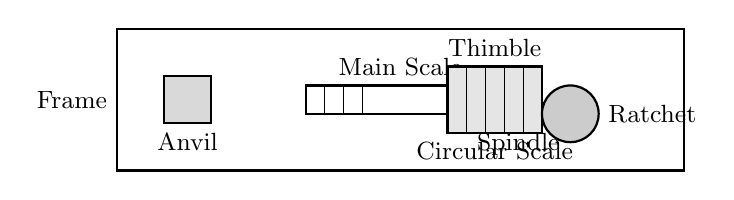
\begin{tikzpicture}[scale=1.2]
    % Frame
    \draw[thick] (0,0) -- (0,1.5) -- (6,1.5) -- (6,0) -- cycle;
    % Anvil
    \fill[gray!30] (0.5,0.5) rectangle (1,1);
    \draw[thick] (0.5,0.5) rectangle (1,1);
    \node[below] at (0.75,0.5) {\small Anvil};
    % Spindle
    \fill[gray!30] (4,0.5) rectangle (4.5,1);
    \draw[thick] (4,0.5) rectangle (4.5,1);
    \node[below] at (4.25,0.5) {\small Spindle};
    % Sleeve (Main Scale)
    \draw[thick] (2,0.6) rectangle (4,0.9);
    \draw (2.2,0.6) -- (2.2,0.9);
    \draw (2.4,0.6) -- (2.4,0.9);
    \draw (2.6,0.6) -- (2.6,0.9);
    \node[above] at (3,0.9) {\small Main Scale};
    % Thimble (Circular Scale)
    \draw[thick,fill=gray!20] (3.5,0.4) rectangle (4.5,1.1);
    \draw (3.7,0.4) -- (3.7,1.1);
    \draw (3.9,0.4) -- (3.9,1.1);
    \draw (4.1,0.4) -- (4.1,1.1);
    \draw (4.3,0.4) -- (4.3,1.1);
    \node[above] at (4,1.1) {\small Thimble};
    \node[below] at (4,0.4) {\small Circular Scale};
    % Ratchet
    \draw[thick,fill=gray!40] (4.8,0.6) circle (0.3);
    \node[right] at (5.1,0.6) {\small Ratchet};
    % Frame label
    \node[left] at (0,0.75) {\small Frame};
\end{tikzpicture}
\caption{Micrometer Screw Gauge}
\end{figure}

\paragraph{Key Parts:}
\begin{enumerate}
    \item \textbf{Frame:} C-shaped rigid body that holds all parts
    \item \textbf{Anvil:} Fixed end against which object is placed
    \item \textbf{Spindle:} Moving part that advances towards anvil
    \item \textbf{Sleeve (Main Scale):} Shows millimeter divisions
    \item \textbf{Thimble (Circular Scale):} Shows fractional divisions (0-50 or 0-100)
    \item \textbf{Ratchet:} Ensures uniform pressure during measurement
\end{enumerate}

\paragraph{Mnemonic:} \emph{Frame-Anvil-Spindle-Sleeve-Thimble-Ratchet (FASSTR).}

\subsection{Question 2(b)(2) [4 marks]}
\textbf{Explain the zero, positive and negative errors for vernier calipers with proper diagram and list necessary steps to remove these types of errors.}

\subsubsection{Solution}
\paragraph{Types of Errors:}

\begin{enumerate}
    \item \textbf{Zero Error:} When the jaws are closed, if the zero of vernier scale does not coincide with zero of main scale, the instrument has zero error.
    
    \item \textbf{Positive Zero Error:} When the zero of vernier scale is to the \textit{right} of the main scale zero. The reading is \textit{more} than actual, so we \textit{subtract} the error.
    
    \item \textbf{Negative Zero Error:} When the zero of vernier scale is to the \textit{left} of the main scale zero. The reading is \textit{less} than actual, so we \textit{add} the error.
\end{enumerate}

\paragraph{Steps to Remove Errors:}
\begin{enumerate}
    \item Note the zero error when jaws are closed
    \item For positive error: Subtract error from measured reading
    \item For negative error: Add the error value to measured reading
    \item Formula: Corrected Reading = Measured Reading - Zero Error
    \item If zero error persists, the instrument needs calibration by a technician
\end{enumerate}

\paragraph{Mnemonic:} \emph{Positive error = Subtract, Negative error = Add.}

\subsection{Question 2(b)(3) [4 marks]}
\textbf{In an experiment of finding the periodic time of a simple pendulum, the observations are 1.96 s, 1.98 s, 2.00 s, 2.02 s, 2.04 s. Calculate absolute error, mean absolute error, relative error and percentage error.}

\subsubsection{Solution}
\paragraph{Given Data:}
Observations: \(T_1 = 1.96\,s\), \(T_2 = 1.98\,s\), \(T_3 = 2.00\,s\), \(T_4 = 2.02\,s\), \(T_5 = 2.04\,s\)

\paragraph{Calculations:}

\subparagraph{Mean Value:}
The mean value is the arithmetic average of all observations:
\[ T_{mean} = \frac{T_1 + T_2 + T_3 + T_4 + T_5}{5} = \frac{1.96 + 1.98 + 2.00 + 2.02 + 2.04}{5} = \frac{10.00}{5} = 2.00\,s \]
This represents the most probable value of the periodic time.

\subparagraph{Absolute Errors:}
Absolute error for each observation is the absolute difference from the mean:
\[ \Delta T_1 = |T_{mean} - T_1| = |2.00 - 1.96| = 0.04\,s \]
\[ \Delta T_2 = |2.00 - 1.98| = 0.02\,s \]
\[ \Delta T_3 = |2.00 - 2.00| = 0.00\,s \]
\[ \Delta T_4 = |2.00 - 2.02| = 0.02\,s \]
\[ \Delta T_5 = |2.00 - 2.04| = 0.04\,s \]

\subparagraph{Mean Absolute Error:}
The mean absolute error is the average of all individual absolute errors:
\[ \Delta T_{mean} = \frac{\Delta T_1 + \Delta T_2 + \Delta T_3 + \Delta T_4 + \Delta T_5}{5} = \frac{0.04 + 0.02 + 0.00 + 0.02 + 0.04}{5} = \frac{0.12}{5} = 0.024\,s \]
This represents the uncertainty in our measurement.

\subparagraph{Relative Error:}
Relative error is the ratio of mean absolute error to mean value:
\[ \text{Relative Error} = \frac{\Delta T_{mean}}{T_{mean}} = \frac{0.024}{2.00} = 0.012 \]
This is a dimensionless quantity that indicates the fractional uncertainty.

\subparagraph{Percentage Error:}
Percentage error expresses relative error as a percentage:
\[ \text{Percentage Error} = \text{Relative Error} \times 100\% = 0.012 \times 100\% = 1.2\% \]

\paragraph{Answers:}
\begin{itemize}
    \item Mean Absolute Error = 0.024 s
    \item Relative Error = 0.012
    \item Percentage Error = 1.2\%
\end{itemize}

\paragraph{Significance:}
A percentage error of 1.2\% indicates high precision in our measurements. The experiment was conducted carefully with minimal random errors.

\paragraph{Mnemonic:} \emph{Mean → Absolute → Relative → Percentage.}

% ========================================
% QUESTION 3: Electromagnetics & Waves (14 marks)
% Q3(A): 3 marks each, Q3(B): 4 marks each
% ========================================

\section{Question 3}

\subsection{Question 3(a)(1) [3 marks]}
\textbf{Define: Electric flux, Electric field, Potential Difference}

\subsubsection{Solution}
\paragraph{Definitions:}

\subparagraph{Electric Flux (\(\Phi_E\)):}
Electric flux through a surface is the total number of electric field lines passing perpendicularly through that surface. Mathematically, \(\Phi_E = \vec{E} \cdot \vec{A} = EA\cos\theta\), where \(\theta\) is the angle between field and area vector. SI unit: \(N \cdot m^2/C\) or \(V \cdot m\).

\subparagraph{Electric Field (\(\vec{E}\)):}
Electric field at a point is the force experienced by a unit positive charge placed at that point. It is defined as \(\vec{E} = \vec{F}/q_0\), where \(q_0\) is a small test charge. SI unit: \(N/C\) or \(V/m\). Direction: away from positive charges, toward negative charges.

\subparagraph{Potential Difference (V):}
Potential difference between two points is the work done per unit charge in moving a small positive charge from one point to another. Mathematically, \(V = W/q\). SI unit: Volt (V) or Joule/Coulomb (J/C). It represents energy per unit charge.

\paragraph{Mnemonic:} \emph{Flux = Field lines, Field = Force/charge, Potential = Work/charge.}

\subsection{Question 3(a)(2) [3 marks]}
\textbf{Derive the formula for equivalent capacitance when three different capacitors are connected in series with necessary circuit diagram.}

\subsubsection{Solution}
\paragraph{Circuit Diagram:}
\begin{figure}[H]
\centering
\begin{tikzpicture}[scale=1]
    \draw (0,0) to[battery, l=V] (0,3);
    \draw (0,3) -- (1,3);
    \draw (1,2.5) -- (1,3.5);
    \draw (1.3,2.7) -- (1.3,3.3);
    \node[above] at (1.15,3.5) {\(C_1\)};
    \draw (1.3,3) -- (3,3);
    \draw (3,2.5) -- (3,3.5);
    \draw (3.3,2.7) -- (3.3,3.3);
    \node[above] at (3.15,3.5) {\(C_2\)};
    \draw (3.3,3) -- (5,3);
    \draw (5,2.5) -- (5,3.5);
    \draw (5.3,2.7) -- (5.3,3.3);
    \node[above] at (5.15,3.5) {\(C_3\)};
    \draw (5.3,3) -- (6,3) -- (6,0) -- (0,0);
\end{tikzpicture}
\caption{Three capacitors in series}
\end{figure}

\paragraph{Derivation:}
For capacitors in series:
\begin{itemize}
    \item Same charge \(Q\) on all capacitors
    \item Total voltage \(V = V_1 + V_2 + V_3\)
    \item For each: \(V_1 = Q/C_1\), \(V_2 = Q/C_2\), \(V_3 = Q/C_3\)
    \item For equivalent: \(V = Q/C_{eq}\)
\end{itemize}

Substituting:
\[ \frac{Q}{C_{eq}} = \frac{Q}{C_1} + \frac{Q}{C_2} + \frac{Q}{C_3} \]
\[ \frac{1}{C_{eq}} = \frac{1}{C_1} + \frac{1}{C_2} + \frac{1}{C_3} \]

\paragraph{Result:}
For \(n\) capacitors in series: \(\frac{1}{C_{eq}} = \sum_{i=1}^{n} \frac{1}{C_i}\)

\paragraph{Mnemonic:} \emph{Series: Add reciprocals (like resistors in parallel).}

\subsection{Question 3(a)(3) [3 marks]}
\textbf{Define: Infrasonic sound, Audible Sound, Ultrasonic sound}

\subsubsection{Solution}
\paragraph{Definitions:}

\subparagraph{Infrasonic Sound:}
Sound waves with frequency below 20 Hz (below human hearing range) are called infrasonic or subsonic sounds. Examples: earthquake waves, whale calls, elephant communication. Humans cannot hear these but can feel vibrations. Used in: seismic studies, animal behavior research.

\subparagraph{Audible Sound:}
Sound waves with frequency between 20 Hz to 20,000 Hz (20 kHz) that can be detected by the normal human ear are called audible sounds. This is the range of human hearing. Most speech occurs between 250 Hz to 6000 Hz. Musical instruments produce sounds in this range.

\subparagraph{Ultrasonic Sound:}
Sound waves with frequency above 20 kHz (above human hearing range) are called ultrasonic sounds. Examples: dog whistles (25 kHz), bat navigation (up to 100 kHz), medical ultrasound (1-18 MHz). Applications: SONAR, medical imaging, cleaning, welding, distance measurement.

\paragraph{Mnemonic:} \emph{Infra \u003c 20 Hz, Audible = 20 Hz - 20 kHz, Ultra \u003e 20 kHz.}

\subsection{Question 3(b)(1) [4 marks]}
\textbf{Prove \(C = \frac{\epsilon_0 A}{d}\) for parallel plate capacitor.}

\subsubsection{Solution}
\paragraph{Configuration:}
Consider a parallel plate capacitor with:
\begin{itemize}
    \item Plate area = \(A\)
    \item Separation between plates = \(d\)
    \item Charge on plates = \(+Q\) and \(-Q\)
    \item Permittivity of free space = \(\epsilon_0\)
\end{itemize}

\paragraph{Derivation:}

\subparagraph{Step 1 - Electric Field:}
For a parallel plate capacitor, the electric field between plates is uniform. Using Gauss's law for a conductor with surface charge density \(\sigma\), the electric field is: \(E = \frac{\sigma}{\epsilon_0} = \frac{Q}{\epsilon_0 A}\)
where \(\sigma = Q/A\) is surface charge density. This field points from positive to negative plate and is constant throughout the space between plates.

\subparagraph{Step 2 - Potential Difference:}
The potential difference between plates is work done per unit charge moving from one plate to another. Since field is uniform:
\(V = Ed = \frac{Qd}{\epsilon_0 A}\)
This relationship shows that voltage increases linearly with plate separation and charge.

\subparagraph{Step 3 - Capacitance:}
By definition, capacitance \(C = \frac{Q}{V}\). Substituting the expression for voltage:
\[ C = \frac{Q}{\frac{Qd}{\epsilon_0 A}} = \frac{Q \epsilon_0 A}{Qd} = \frac{\epsilon_0 A}{d} \]

\paragraph{Result:}
\[ \boxed{C = \frac{\epsilon_0 A}{d}} \]

This shows capacitance is:
\begin{itemize}
    \item Directly proportional to plate area \(A\): Larger area stores more charge
    \item Inversely proportional to separation \(d\): Closer plates create stronger field
    \item Independent of charge \(Q\) or voltage \(V\): Capacitance is geometric property
\end{itemize}

\paragraph{Mnemonic:} \emph{C = \(\epsilon\)A/d (Epsilon-Area/distance).}

\subsection{Question 3(b)(2) [4 marks]}
\textbf{List the characteristics of electric field lines.}

\subsubsection{Solution}
\paragraph{Characteristics of Electric Field Lines:}

\begin{enumerate}
    \item \textbf{Origin and Termination:} Electric field lines originate from positive charges and terminate on negative charges. In absence of negative charges, they extend to infinity.
    
    \item \textbf{Direction:} The tangent to a field line at any point gives the direction of electric field at that point. Field points away from +ve and toward -ve charges.
    
    \item \textbf{No Intersection:} Two electric field lines never intersect each other. If they did, at the point of intersection there would be two directions of electric field, which is impossible.
    
    \item \textbf{Density and Strength:} The number of field lines per unit area (density) is proportional to the magnitude of electric field. Closer lines indicate stronger field.
    
    \item \textbf{Perpendicularity:} Electric field lines are always perpendicular to the surface of a conductor at equilibrium. Inside a conductor, electric field is zero.
    
    \item \textbf{Continuity:} Field lines are continuous curves without any breaks. They do not start or end in empty space (except at infinity).
    
    \item \textbf{Symmetry:} For symmetric charge distributions, field lines show corresponding symmetry. Example: radial lines for point charge, parallel lines for infinite plane.
    
    \textbf{Not Physical:} Field lines are imaginary lines used for visualization. They do not represent actual physical trajectories of charges.
\end{enumerate}

\begin{figure}[H]
\centering
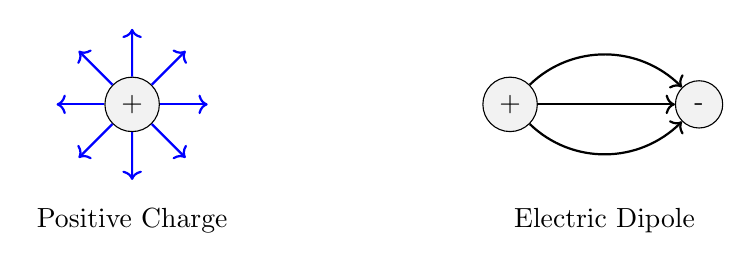
\begin{tikzpicture}[scale=0.8]
    % Positive Charge at left
    \node[circle,draw,fill=gray!10,minimum size=0.6cm] (P) at (-3,0) {+};
    \foreach \angle in {0,45,...,315}
        \draw[->,thick,blue] (P) -- ++(\angle:1.2cm);
    \node[below] at (-3,-1.5) {Positive Charge};
    % Dipole at right
    \begin{scope}[xshift=3cm]
    \node[circle,draw,fill=gray!10,minimum size=0.6cm] (P2) at (0,0) {+};
    \node[circle,draw,fill=gray!10,minimum size=0.6cm] (N2) at (3,0) {-};
    \draw[->,thick] (P2) -- (N2);
    \draw[->,thick] (P2) to[bend left=45] (N2);
    \draw[->,thick] (P2) to[bend right=45] (N2);
    \node[below] at (1.5,-1.5) {Electric Dipole};
    \end{scope}
\end{tikzpicture}
\caption{Electric Field Lines}
\end{figure}

\paragraph{Mnemonic:} \emph{+ve to -ve, Never cross, Density = Strength, Perpendicular to surfaces.}

\subsection{Question 3(b)(3) [4 marks]}
\textbf{Describe working and construction of magnetostriction method used for production of ultrasonic waves.}

\subsubsection{Solution}
\paragraph{Principle:}
Magnetostriction is the property of ferromagnetic materials (iron, nickel, cobalt) to change their dimensions when placed in a magnetic field. When the field changes, the material expands or contracts, producing mechanical vibrations.

\paragraph{Construction Diagram:}
\begin{figure}[H]
\centering
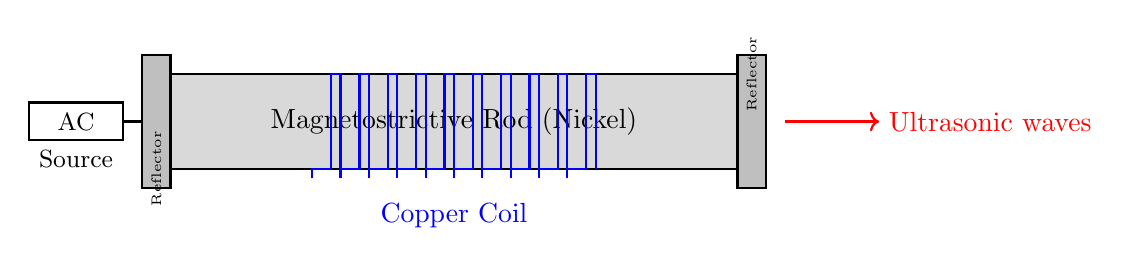
\begin{tikzpicture}[scale=1.2]
    % Rod
    \draw[thick,fill=gray!30] (0,0.5) rectangle (6,1.5);
    \node at (3,1) {Magnetostrictive Rod (Nickel)};
    % Coil windings
    \foreach \x in {1.5,1.8,...,4.5} {
        \draw[thick,blue] (\x,0.4) -- (\x,0.5) -- (\x+0.2,0.5) -- (\x+0.2,1.5) -- (\x+0.3,1.5) -- (\x+0.3,0.5);
    }
    \node[blue] at (3,0) {Copper Coil};
    % AC Source
    \draw[thick] (0,1) -- (-0.5,1);
    \draw[thick] (-0.5,0.8) rectangle (-1.5,1.2);
    \node at (-1,1) {\small AC};
    \node[below] at (-1,0.8) {\small Source};
    % Reflector plates
    \draw[thick,fill=gray!50] (-0.3,0.3) rectangle (0,1.7);
    \draw[thick,fill=gray!50] (6,0.3) rectangle (6.3,1.7);
    \node[left,rotate=90] at (-0.15,1) {\tiny Reflector};
    \node[right,rotate=90] at (6.15,1) {\tiny Reflector};
    % Waves
    \draw[->,thick,red] (6.5,1) -- (7.5,1);
    \node[red,right] at (7.5,1) {Ultrasonic waves};
\end{tikzpicture}
\caption{Magnetostriction Ultrasonic Generator}
\end{figure}

\paragraph{Construction Components:}
\begin{itemize}
    \item \textbf{Magnetostrictive Rod:} Ferromagnetic material rod (nickel or iron-nickel alloy) that vibrates
    \item \textbf{Coil:} Insulated copper wire wound around the rod to create magnetic field
    \item \textbf{AC Source:} High-frequency alternating current (20-100 kHz) power supply
    \item \textbf{Reflector Plates:} Metal plates at ends to reflect and concentrate ultrasonic waves
\end{itemize}

\paragraph{Working:}
\begin{enumerate}
    \item AC current flows through the coil, creating an alternating magnetic field
    \item The magnetostrictive rod undergoes periodic expansion and contraction at the frequency of AC
    \item When frequency matches the natural frequency of the rod (resonance), maximum vibrations occur
    \item These mechanical vibrations produce ultrasonic waves in the surrounding medium
    \item The rod length \(L\) is chosen such that \(L = n\lambda/2\) for resonance
\end{enumerate}

\paragraph{Advantages:}
High power ultrasonic waves, simple construction, reliable operation.

\paragraph{Disadvantages:}
Limited to lower ultrasonic frequencies (\u003c 100 kHz), efficiency decreases at higher frequencies, heating of rod.

\paragraph{Applications:}
Ultrasonic cleaning, drilling, welding, SONAR systems.

\paragraph{Mnemonic:} \emph{Magnetic field → Dimension change → Vibrations → Ultrasound.}

% ========================================
% QUESTION 4: Optics & Fibers (14 marks)
% Q4(A): 3 marks each, Q4(B): 4 marks each
% ========================================

\section{Question 4}

\subsection{Question 4(a)(1) [3 marks]}
\textbf{A radio station broadcasts its radio signals at 100 MHz. Find the wavelength if the waves travel at a speed of \(3 \times 10^8\,m/s\).}

\subsubsection{Solution}
\paragraph{Given Data:}
\begin{itemize}
    \item Frequency, \(f = 100\,MHz = 100 \times 10^6\,Hz = 10^8\,Hz\)
    \item Speed of wave, \(v = 3 \times 10^8\,m/s\)
\end{itemize}

\paragraph{Formula:}
The fundamental relationship between wave speed, frequency, and wavelength for all electromagnetic waves is:
\[ v = f\lambda \]
where \(v\) is wave speed in m/s, \(f\) is frequency in Hz, and \(\lambda\) (lambda) is wavelength in meters. This equation shows that wavelength and frequency are inversely proportional for a given wave speed. Higher frequency means shorter wavelength and vice versa.

\paragraph{Calculation:}
Rearranging the formula to find wavelength:
\[ \lambda = \frac{v}{f} = \frac{3 \times 10^8\,m/s}{10^8\,Hz} = 3\,m \]

\paragraph{Answer:}
The wavelength of radio signals is \textbf{3 meters}. This is in the radio wave region of the electromagnetic spectrum, ideal for broadcasting because: (1) these waves can travel long distances through atmosphere, (2) they can penetrate buildings and obstacles, (3) they require reasonably-sized antennas (quarter-wavelength = 75 cm), and (4) they have good diffraction properties around obstacles.

\paragraph{Mnemonic:} \emph{\(\lambda\) = v/f (wavelength = speed/frequency).}

\subsection{Question 4(a)(2) [3 marks]}
\textbf{State the Snell's law and explain refractive index of media.}

\subsubsection{Solution}
\paragraph{Snell's Law:}
\begin{figure}[H]
\centering
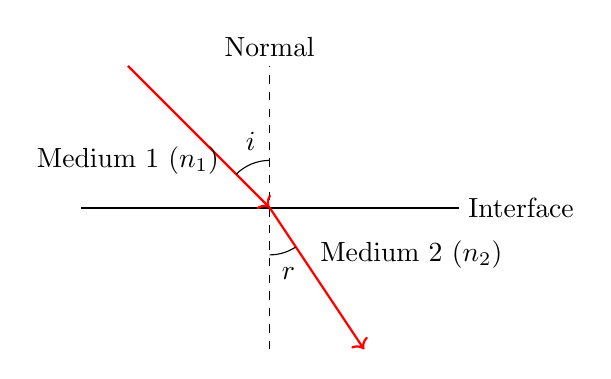
\begin{tikzpicture}[scale=1.2]
    % Interface
    \draw[thick] (-2,0) -- (2,0);
    \node[right] at (2,0) {Interface};
    % Normal
    \draw[dashed] (0,-1.5) -- (0,1.5);
    \node[above] at (0,1.5) {Normal};
    % Rays
    \draw[thick,red,->] (-1.5,1.5) -- (0,0);
    \draw[thick,red,->] (0,0) -- (1,-1.5);
    % Angles
    \draw (0,0.5) arc (90:135:0.5); \node at (-0.2,0.7) {\(i\)};
    \draw (0,-0.5) arc (270:303:0.5); \node at (0.2,-0.7) {\(r\)};
    % Media
    \node at (-1.5,0.5) {Medium 1 (\(n_1\))};
    \node at (1.5,-0.5) {Medium 2 (\(n_2\))};
\end{tikzpicture}
\caption{Refraction (Snell's Law)}
\end{figure}
When a light ray passes from one medium to another, the ratio of sine of angle of incidence to sine of angle of refraction is constant. Mathematically:
\[ \frac{\sin i}{\sin r} = \text{constant} = \frac{n_2}{n_1} \]
Or: \( n_1 \sin i = n_2 \sin r \)

where \(i\) is angle of incidence, \(r\) is angle of refraction, \(n_1\) and \(n_2\) are refractive indices of medium 1 and 2.

\paragraph{Refractive Index:}
The refractive index (\(n\)) of a medium is defined as the ratio of speed of light in vacuum to speed of light in that medium:
\[ n = \frac{c}{v} \]

where \(c = 3 \times 10^8\,m/s\) is speed of light in vacuum, and \(v\) is speed of light in the medium. Refractive index is dimensionless and always \(\geq 1\). Greater refractive index means light travels slower in that medium and bends more towards normal when entering from a rarer medium.

\paragraph{Examples:}
\begin{itemize}
    \item Air: \(n \approx 1.0003 \approx 1\)
    \item Water: \(n \approx 1.33\)
    \item Glass: \(n \approx 1.5\)
    \item Diamond: \(n \approx 2.42\)
\end{itemize}

\paragraph{Mnemonic:} \emph{n\(_1\)sin(i) = n\(_2\)sin(r), n = c/v.}

\subsection{Question 4(a)(3) [3 marks]}
\textbf{Compare: Ordinary light and LASER}

\subsubsection{Solution}
\paragraph{Comparison Table:}
\begin{table}[H]
\caption{Ordinary Light vs LASER}
\centering
\begin{tabularx}{\textwidth}{|X|X|}
\hline
\textbf{Ordinary Light} & \textbf{LASER} \\ \hline
Polychromatic (many wavelengths) & Monochromatic (single wavelength) \\ \hline
Incoherent (random phase) & Coherent (constant phase relationship) \\ \hline
Divergent beam (spreads out) & Highly directional (parallel beam) \\ \hline
Low intensity & Very high intensity \\ \hline
Example: Bulb, sunlight & Example: He-Ne laser, CO\(_2\) laser \\ \hline
Uses: General lighting & Uses: Surgery, cutting, communication \\ \hline
\end{tabularx}
\end{table}

\paragraph{Key Differences:}
\begin{enumerate}
    \item \textbf{Monochromaticity:} LASER emits single color/wavelength, ordinary light has mix of colors
    \item \textbf{Coherence:} LASER waves are in phase, ordinary light waves have random phase
    \item \textbf{Directionality:} LASER is highly directional, ordinary light spreads in all directions
    \item \textbf{Intensity:} LASER has concentrated high intensity, ordinary light has low intensity
\end{enumerate}

\paragraph{Mnemonic:} \emph{LASER = Monochromatic + Coherent + Directional + Intense.}

\subsection{Question 4(b)(1) [4 marks]}
\textbf{Demonstrate the structure of an optical fiber with necessary diagram.}

\subsubsection{Solution}
\paragraph{Structure Diagram:}
\begin{figure}[H]
\centering
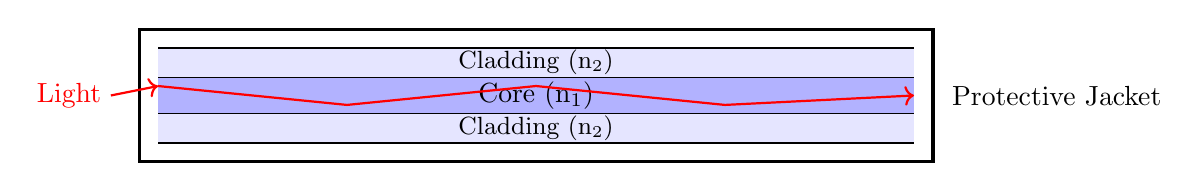
\begin{tikzpicture}[scale=1.2]
    % Core
    \fill[blue!30] (0,0.3) rectangle (8,0.7);
    \draw[thick] (0,0.3) -- (8,0.3);
    \draw[thick] (0,0.7) -- (8,0.7);
    \node at (4,0.5) {Core (n\(_1\))};
    % Cladding
    \fill[blue!10] (0,0) rectangle (8,0.3);
    \fill[blue!10] (0,0.7) rectangle (8,1);
    \draw[thick] (0,0) -- (8,0);
    \draw[thick] (0,1) -- (8,1);
    \node at (4,0.15) {\small Cladding (n\(_2\))};
    \node at (4,0.85) {\small Cladding (n\(_2\))};
    % Jacket
    \draw[very thick] (-0.2,-0.2) rectangle (8.2,1.2);
   \node[right] at (8.3,0.5) {Protective Jacket};
    % Light ray
    \draw[->,red,thick] (-0.5,0.5) -- (0,0.6);
    \draw[->,red,thick] (0,0.6) -- (2,0.4) -- (4,0.6) -- (6,0.4) -- (8,0.5);
    \node[red,left] at (-0.5,0.5) {Light};
\end{tikzpicture}
\caption{Optical Fiber Structure}
\end{figure}

\paragraph{Components:}
\begin{enumerate}
    \item \textbf{Core:} Central cylinder with high refractive index (\(n_1\)). Light travels through core by total internal reflection. Diameter: 8-10 \(\mu\)m (single mode) or 50-100 \(\mu\)m (multimode).
    
    \item \textbf{Cladding:} Surrounds core with lower refractive index (\(n_2 < n_1\)). Ensures total internal reflection and prevents light leakage. Thickness: 125 \(\mu\)m typically.
    
    \item \textbf{Protective Jacket:} Outer polymer coating protects fiber from physical damage, moisture, and mechanical stress.
\end{enumerate}

\paragraph{Working Principle:}
Light travels through core via total internal reflection at core-cladding boundary. Condition: \(n_1 > n_2\) and angle of incidence \(> \) critical angle.

\paragraph{Mnemonic:} \emph{Core (high n) + Cladding (low n) + Jacket = Fiber.}

\subsection{Question 4(b)(2) [4 marks]}
\textbf{List applications of LASER in engineering and medical field.}

\subsubsection{Solution}
\paragraph{Engineering Applications:}
\begin{enumerate}
    \item \textbf{Material Processing:} Laser cutting, welding, drilling of metals and plastics with high precision
    \item \textbf{Communication:} Fiber optic communication for high-speed data transmission over long distances
    \item \textbf{Measurement:} Distance measurement (LIDAR), alignment in construction, surveying
    \item \textbf{Manufacturing:} 3D printing, laser engraving, surface treatment and hardening
    \item \textbf{Holography:} Creating 3D holograms for security and display applications
    \item \textbf{Barcode Scanning:} Retail checkout systems and inventory management
    \item \textbf{Defense:} Laser guided missiles, range finders, target designation
\end{enumerate}

\paragraph{Medical Applications:}
\begin{enumerate}
    \item \textbf{Surgery:} Laser scalpel for bloodless cutting, precise tissue removal
    \item \textbf{Ophthalmology:} LASIK eye surgery for vision correction, retinal repair
    \item \textbf{Dermatology:} Tattoo removal, skin resurfacing, hair removal
    \item \textbf{Dentistry:} Cavity treatment, gum surgery, teeth whitening
    \item \textbf{Cancer Treatment:} Tumor removal, photodynamic therapy
    \item \textbf{Diagnosis:} Laser microscopy, blood analysis, tissue imaging
    \item \textbf{Cosmetic:} Wrinkle reduction, scar treatment
\end{enumerate}

\paragraph{Advantages:}
High precision, minimal bleeding, faster healing, reduced infection risk, non-contact operation.

\paragraph{Mnemonic:} \emph{Engineering: Cut-Weld-Communicate-Measure. Medical: Surgery-Eye-Skin-Cancer.}

\subsection{Question 4(b)(3) [4 marks]}
\textbf{Explain P-type and N-type semiconductors.}

\subsubsection{Solution}
\paragraph{N-Type Semiconductor:}
\begin{itemize}
    \item \textbf{Doping:} Pure semiconductor (Si or Ge) doped with pentavalent impurity (P, As, Sb)
    \item \textbf{Majority Carriers:} Electrons (free electrons from donor atoms)
    \item \textbf{Minority Carriers:} Holes
    \item \textbf{Donor Atoms:} Pentavalent atoms donate extra electron
    \item \textbf{Charge:} Electrically neutral overall but electron-rich
\end{itemize}

\paragraph{P-Type Semiconductor:}
\begin{itemize}
    \item \textbf{Doping:} Pure semiconductor doped with trivalent impurity (B, Al, Ga, In)
    \item \textbf{Majority Carriers:} Holes (absence of electrons)
    \item \textbf{Minority Carriers:} Electrons
    \item \textbf{Acceptor Atoms:} Trivalent atoms accept electrons, creating holes
    \item \textbf{Charge:} Electrically neutral overall but hole-rich
\end{itemize}

\paragraph{Comparison:}
\begin{itemize}
    \item N-type has excess electrons, P-type has excess holes
    \item N-type uses Group V elements, P-type uses Group III elements
    \item Both are electrically neutral
    \item Conductivity of both is higher than pure semiconductor
\end{itemize}

\paragraph{Applications:}
Used to form PN junctions in diodes, transistors, solar cells, LEDs, and other semiconductor devices.

\paragraph{Mnemonic:} \emph{N = Negative carriers (electrons), P = Positive carriers (holes).}

% ========================================
% QUESTION 5: Semiconductors & Logic (14 marks)
% Q5(A): 3 marks each, Q5(B): 4 marks each
% ========================================

\section{Question 5}

\subsection{Question 5(a)(1) [3 marks]}
\textbf{Classify conductors, semiconductors and insulators based on energy band gap.}

\subsubsection{Solution}
\paragraph{Classification Table:}
\begin{table}[H]
\caption{Classification based on Energy Band Gap}
\centering
\begin{tabularx}{\textwidth}{|X|X|X|X|}
\hline
\textbf{Type} & \textbf{Band Gap (E\(_g\))} & \textbf{Example} & \textbf{Conductivity} \\ \hline
Conductors & No band gap (E\(_g\) = 0) & Cu, Ag, Al, Au & Very high (\(10^7\,S/m\)) \\ \hline
Semiconductors & Small gap (0.1 to 3 eV) & Si (1.1 eV), Ge (0.7 eV) & Moderate (\(10^{-4}\) to \(10^4\,S/m\)) \\ \hline
Insulators & Large gap (\(>3\) eV) & Diamond (5.5 eV), Glass & Very low (\(10^{-15}\,S/m\)) \\ \hline
\end{tabularx}
\end{table}

\begin{figure}[H]
\centering
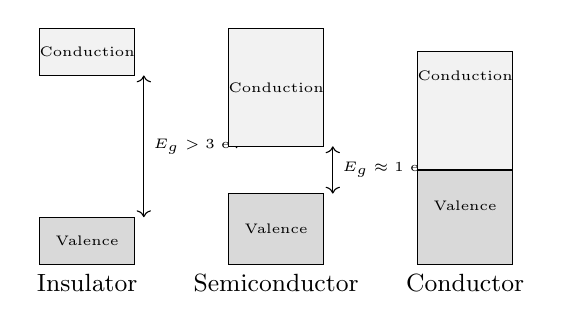
\begin{tikzpicture}[scale=0.6]
    % Insulator
    \draw[fill=gray!30] (0,0) rectangle (2,1) node[midway] {\tiny Valence};
    \draw[fill=gray!10] (0,4) rectangle (2,5) node[midway] {\tiny Conduction};
    \draw[<->] (2.2,1) -- (2.2,4) node[midway,right] {\tiny \(E_g > 3\) eV};
    \node[below] at (1,0) {\small Insulator};
    % Semiconductor
    \begin{scope}[xshift=4cm]
    \draw[fill=gray!30] (0,0) rectangle (2,1.5) node[midway] {\tiny Valence};
    \draw[fill=gray!10] (0,2.5) rectangle (2,5) node[midway] {\tiny Conduction};
    \draw[<->] (2.2,1.5) -- (2.2,2.5) node[midway,right] {\tiny \(E_g \approx 1\) eV};
    \node[below] at (1,0) {\small Semiconductor};
    \end{scope}
    % Conductor
    \begin{scope}[xshift=8cm]
    \draw[fill=gray!30] (0,0) rectangle (2,2.5) node[midway] {\tiny Valence};
    \draw[fill=gray!10] (0,2) rectangle (2,4.5);
    \node at (1,4) {\tiny Conduction};
    \node[below] at (1,0) {\small Conductor};
    \end{scope}
\end{tikzpicture}
\caption{Energy Band Comparison}
\end{figure}

\paragraph{Detailed Description:}
\begin{enumerate}
    \item \textbf{Conductors:} Valence and conduction bands overlap. Electrons can move freely without needing extra energy. High conductivity at all temperatures.
    
    \item \textbf{Semiconductors:} Small forbidden energy gap. At room temperature, thermal energy provides enough excitation for some electrons to jump to conduction band. Conductivity increases with temperature.
    
    \item \textbf{Insulators:} Very large energy gap. Electrons cannot easily jump to conduction band even at high temperatures. Remain poor conductors.
\end{enumerate}

\paragraph{Mnemonic:} \emph{Conductors: Zero gap. Semiconductors: Small gap. Insulators: Large gap.}

\subsection{Question 5(a)(2) [3 marks]}
\textbf{Explain OR and AND logic gates with necessary truth table.}

\subsubsection{Solution}
\begin{figure}[H]
\centering
\begin{circuitikz}[scale=1]
    % OR Gate
    \draw (0,2) node[or port] (OR) {};
    \node[left] at (OR.in 1) {A};
    \node[left] at (OR.in 2) {B};
    \node[right] at (OR.out) {Y};
    \node[below] at (OR.south) {OR Gate};

    % AND Gate
    \draw (5,2) node[and port] (AND) {};
    \node[left] at (AND.in 1) {A};
    \node[left] at (AND.in 2) {B};
    \node[right] at (AND.out) {Y};
    \node[below] at (AND.south) {AND Gate};
\end{circuitikz}
\caption{Logic Gate Symbols}
\end{figure}
\paragraph{OR Gate:}
Output is HIGH (1) if ANY input is HIGH.

\textbf{Truth Table:}
\begin{table}[H]
\caption{OR Gate Truth Table}
\centering
\begin{tabularx}{0.7\textwidth}{|X|X|X|}
\hline
\textbf{A} & \textbf{B} & \textbf{Y = A + B} \\ \hline
0 & 0 & 0 \\ \hline
0 & 1 & 1 \\ \hline
1 & 0 & 1 \\ \hline
1 & 1 & 1 \\ \hline
\end{tabularx}
\end{table}

\textbf{Boolean Expression:} \( Y = A + B \)

\paragraph{AND Gate:}
Output is HIGH (1) only if ALL inputs are HIGH.

\textbf{Truth Table:}
\begin{table}[H]
\caption{AND Gate Truth Table}
\centering
\begin{tabularx}{0.7\textwidth}{|X|X|X|}
\hline
\textbf{A} & \textbf{B} & \textbf{Y = A · B} \\ \hline
0 & 0 & 0 \\ \hline
0 & 1 & 0 \\ \hline
1 & 0 & 0 \\ \hline
1 & 1 & 1 \\ \hline
\end{tabularx}
\end{table}

\textbf{Boolean Expression:} \( Y = A \cdot B \) or \( Y = AB \)

\paragraph{Summary:}
OR gate: Addition operation, AND gate: Multiplication operation. Both are fundamental gates used in digital circuit design.

\paragraph{Mnemonic:} \emph{OR = Any HIGH gives HIGH. AND = All HIGH gives HIGH.}

\subsection{Question 5(a)(3) [3 marks]}
\textbf{Describe the use of Zener diode as a voltage regulator.}

\subsubsection{Solution}
\paragraph{Principle:}
Zener diode operates in reverse bias breakdown region. It maintains constant voltage across its terminals despite changes in current. This property makes it ideal for voltage regulation.

\paragraph{Working:}
\begin{enumerate}
    \item Zener diode is connected in reverse bias parallel to load
    \item Series resistor \(R_s\) is connected to limit current
    \item When input voltage increases, Zener current increases but voltage remains constant at \(V_Z\)
    \item When input decreases (but stays above \(V_Z\)), Zener adjusts current to maintain constant output
    \item Load receives stable voltage equal to Zener breakdown voltage
\end{enumerate}

\paragraph{Applications:}
\begin{itemize}
    \item Power supply voltage stabilization
    \item Protection of sensitive electronic components
    \item Reference voltage generation
    \item Voltage limiting circuits
\end{itemize}

\paragraph{Advantages:}
Simple, low cost, reliable, fast response.

\paragraph{Limitations:}
Limited power handling, not suitable for variable output voltage.

\paragraph{Mnemonic:} \emph{Zener in reverse bias = Constant voltage regulator.}

\subsection{Question 5(b)(1) [4 marks]}
\textbf{Explain full wave rectifier with necessary circuit and draw input and output waveforms.}

\subsubsection{Solution}
\paragraph{Circuit Configuration:}
Full wave rectifier uses a center-tapped transformer with two diodes (D\(_1\) and D\(_2\)) connected to convert alternating current (AC) into pulsating direct current (DC). The center tap of secondary winding is grounded, creating two equal voltage sources of opposite polarity. Load resistor is connected between center tap and cathodes of both diodes.

\paragraph{Working Principle:}
\begin{itemize}
    \item \textbf{Positive Half Cycle:} Upper terminal is positive. Diode D\(_1\) becomes forward biased and conducts while D\(_2\) is reverse biased and blocks. Current flows through load from ground to upper terminal.
    \item \textbf{Negative Half Cycle:} Lower terminal is positive. Diode D\(_2\) becomes forward biased and conducts while D\(_1\) is reverse biased and blocks. Current flows through load in SAME direction from ground to lower terminal.
    \item Both half cycles produce output current in same direction through load, hence ``full wave' rectification. This is key advantage over half wave rectifier which uses only one half cycle.
\end{itemize}

\paragraph{Characteristics:}
\begin{itemize}
    \item Efficiency: 81.2\% (much better than half wave's 40.6\%)
    \item Ripple frequency: \(2f\) (double the input frequency, easier to filter)
    \item Output voltage: \(V_{dc} = \frac{2V_m}{\pi} \approx 0.636V_m\)
    \item Peak Inverse Voltage (PIV): \(2V_m\) (each diode must withstand)
    \item Better transformer utilization factor than half wave
\end{itemize}

\paragraph{Advantages:}
Higher efficiency (81.2\%), better ripple factor (lower ripple), higher DC output voltage, better transformer utilization, easier filtering due to higher ripple frequency.

\paragraph{Disadvantages:}
Requires center-tapped transformer (more expensive), uses only half of transformer secondary at a time, higher PIV rating needed for diodes.

\paragraph{Applications:}
DC power supplies for electronic circuits, battery chargers, signal demodulation in AM radio receivers, voltage regulators.

\paragraph{Mnemonic:} \emph{Full wave = Both halves utilized, 2 diodes, 81\% efficiency.}

\subsection{Question 5(b)(2) [4 marks]}
\textbf{Demonstrate forward and reverse characteristics of P-N junction diode.}

\subsubsection{Solution}
\paragraph{Forward Bias Characteristics:}
\begin{itemize}
    \item P-side connected to positive, N-side to negative
    \item Depletion region narrows, barrier potential reduces
    \item \textbf{Cut-in/Threshold Voltage:} Si: 0.7V, Ge: 0.3V
    \item Below cut-in: Negligible current (few \(\mu\)A)
    \item Above cut-in: Current increases exponentially
    \item Forward resistance: Very low (few ohms)
\end{itemize}

\begin{figure}[H]
\centering
\begin{tikzpicture}[scale=0.8]
    \draw[->] (-3,0) -- (3,0) node[right] {\(V\)};
    \draw[->] (0,-2) -- (0,3) node[above] {\(I\)};
    \draw[thick,blue] (0,0) -- (0.5,0) .. controls (1,0.1) and (1.2,1) .. (1.5,2.8);
    \node[blue,right] at (1.5,2) {Fwd Bias};
    \draw[thick,red] (0,0) -- (-1,-0.1) -- (-2.5,-1.8);
    \node[red,left] at (-1,-1) {Rev Bias};
\end{tikzpicture}
\caption{IV Characteristics}
\end{figure}

\paragraph{Reverse Bias Characteristics:}
\begin{itemize}
    \item P-side connected to negative, N-side to positive
    \item Depletion region widens, barrier potential increases
    \item \textbf{Reverse Saturation Current:} Very small (few \(\mu\)A to nA)
    \item Remains nearly constant for wide voltage range
    \item \textbf{Breakdown Voltage:} Beyond certain reverse voltage, current increases sharply
    \item Reverse resistance: Very high (several M\(\Omega\))
\end{itemize}

\paragraph{Key Points:}
\begin{itemize}
    \item Diode conducts easily in forward bias, blocks in reverse bias
    \item Ratio of forward to reverse resistance: \(10^6\) to \(10^8\)
    \item Acts as one-way valve for current
\end{itemize}

\paragraph{Applications:}
Rectifiers, clipping circuits, clamping circuits, voltage regulators.

\paragraph{Mnemonic:} \emph{Forward = Low R, High I. Reverse = High R, Low I.}

\subsection{Question 5(b)(3) [4 marks]}
\textbf{Write the principle of LED and explain its construction and working.}

\subsubsection{Solution}
\paragraph{Principle:}
Light Emitting Diode (LED) works on principle of electroluminescence. When P-N junction is forward biased, electrons and holes recombine, releasing energy as photons (light). Energy of photon determines color: \(E = hf = \frac{hc}{\lambda}\).

\paragraph{Construction:}
\begin{itemize}
    \item P-N junction made of compound semiconductors (GaAs, GaP, GaAsP, GaN)
    \item Transparent epoxy resin dome acts as lens
    \item Reflector cup to direct light upward
    \item Metal contacts for anode (+) and cathode (-)
    \item Longer lead is anode, shorter is cathode
\end{itemize}

\paragraph{Working:}
\begin{enumerate}
    \item LED is forward biased (anode to +ve, cathode to -ve)
    \item Electrons from N-region and holes from P-region move towards junction
    \item At junction, recombination occurs
    \item Energy released as photons (light)
    \item Color depends on semiconductor material's band gap
\end{enumerate}

\paragraph{LED Colors:}
\begin{itemize}
    \item Red: GaAsP (1.8 eV)
    \item Green: GaP (2.2 eV)
    \item Blue: GaN (2.9 eV)
    \item White: Blue LED + Yellow phosphor coating
\end{itemize}

\paragraph{Advantages:}
Long life (50,000+ hours), low power consumption, fast switching, compact size, durable, no mercury.

\paragraph{Applications:}
Displays, indicators, traffic lights, automotive lighting, street lights, backlighting.

\paragraph{Mnemonic:} \emph{LED = Forward bias → Recombination → Photon emission → Light!}

\end{document}

